\section{System Model}\label{sec:model}
\subsection{Network and organisation}
The area is tiled by hexagonal cells of radius $R_{\mathrm c}=100$\,m. The static nodes form an IEEE 802.15.4 mesh that
is organised once, before any mission (\emph{phase~0}): every cell has a cell leader (CL); two adjacent cells are joined
by exactly one gateway pair; cell channels follow a 7-colour reuse and every gateway pair has its own radio and channel;
cell-level routes are precomputed. Cells are grouped into clusters of at most 80 cells, each with a cluster head (CH) that
has a LoRa uplink to the BS. Let $G=(V,E)$ be the graph whose vertices are cells and whose edges are gateway pairs. A
subset $K\subseteq V$ of \emph{critical cells} hosts an AI node (a smart camera or an edge box); the other cameras are
legacy devices that detect motion and keep event crops in a ring buffer.

\subsection{UAVs and emission}
Team~1 is a fixed-wing UAV at altitude $h=100$\,m with speed $v\in[25,50]$\,m/s and bank angle at most $45^\circ$, hence a
turning radius $\rho(v)=v^2/g$: 255\,m at 50\,m/s and 63.7\,m at 25\,m/s. It broadcasts one packet of $B=99$\,B payload
every $\Tp=10$\,ms, i.e., every $\Delta=v\Tp\le 0.5$\,m. Its ground track is a curve $\gamma$ from and to the BS; packet
$s$ is emitted at $x_s=\gamma(s\Tp)$. Team~2 is a rotary-wing UAV (15\,m/s) that verifies candidate cells in phase~2.

\subsection{Air-to-ground reception}
At slant distance $\ell=\sqrt{d^2+h^2}$ the path loss is free space up to $d_0=100$\,m ($PL_0=80.05$\,dB at 2.4\,GHz)
and grows with exponent $\alpha=3$ beyond, plus an excess loss $L_{\mathrm{obs}}$ of the environment:
\begin{equation}
PL(\ell)=PL_0+10\alpha\log_{10}(\ell/d_0)+L_{\mathrm{obs}},\qquad \ell\ge d_0 .\label{eq:pl}
\end{equation}
Each packet sees independent Rician fading with $K=2$ (Nakagami $m=1.8$ in ns-3) and is received when the faded power
exceeds an effective threshold $S$. With $P_{\mathrm t}=10$\,dBm, a node at horizontal distance $d$ receives a packet with
probability
\begin{equation}
p(d)=\Pr\bigl\{g>10^{(S-P_{\mathrm t}+PL(\ell))/10}\bigr\},\quad 2(K{+}1)g\sim\chi'^2_2(2K).\label{eq:pd}
\end{equation}
We summarise a regime by $R_{50}$, the horizontal distance at which $p=1/2$. The four regimes of this paper,
$L_{\mathrm{obs}}=0$, 9.0, 19.8 and 25.7\,dB, give $R_{50}=1016$, 498, 199 and 99\,m. A single threshold
$S=-101.04$\,dBm (nominal sensitivity $-100$\,dBm) reproduces the reception measured on the ns-3 passes in all four
regimes with a root-mean-square error of at most 0.003 (Fig.~\ref{fig:channel}).

The CL gathers what the nodes of its cell hold, so the relevant event is that \emph{some} node of the cell hears the
packet. For a cell $k$ with node set $U_k$ and a UAV at horizontal position $x$,
\begin{equation}
P_k(x)=1-\prod_{u\in U_k}\bigl(1-p(\lVert x-u\rVert)\bigr).\label{eq:pcell}
\end{equation}
Equation~\eqref{eq:pcell} assumes independent receptions across nodes (A1). The limits of Section~\ref{sec:limits} need
only the marginal probabilities $P_k(x)$ and no independence across packets.

\begin{figure}[t]\centering
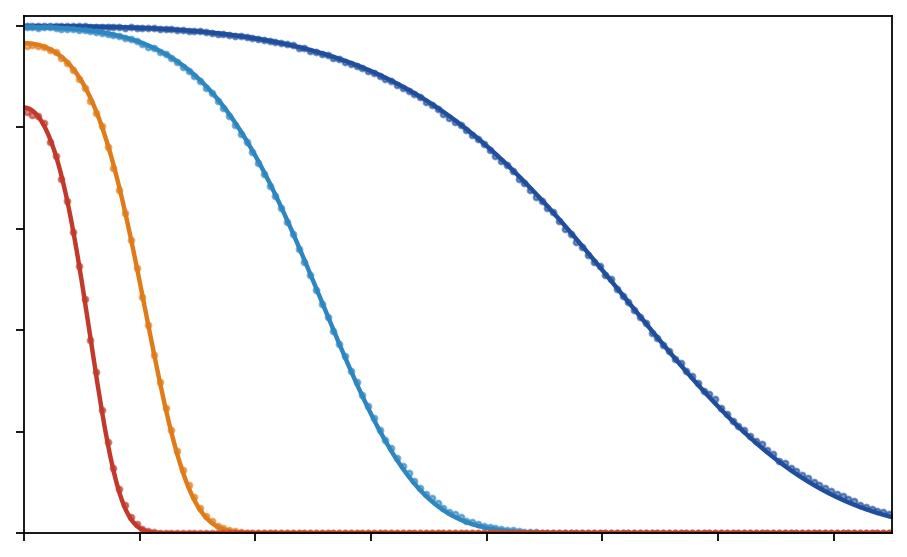
\includegraphics[width=0.86\columnwidth]{nd1-channel-p-of-d-model-vs-ns3.png}
\caption{Packet reception versus horizontal distance (0 to 1.5\,km; vertical axis 0 to 1) for the four regimes, from
$R_{50}=1016$\,m (rightmost) to 99\,m. Dots: measured on ns-3 passes in 10\,m bins. Lines: model \eqref{eq:pd} with one
common threshold. \todo{labelled version of this plot}}\label{fig:channel}
\end{figure}

\subsection{Ground medium}
Ground links follow exponent 3.5 with log-normal shadowing ($\sigma=7.8$\,dB, drawn once per node pair) and Rayleigh
fading in 100\,ms blocks \cite{tr38901}. Every cell and every gateway pair is one \emph{medium}: at most one of its
radios transmits at a time, under CSMA/CA with acknowledgements and retransmissions. An acknowledged hop of a 127\,B frame
occupies its medium for at least $\tau_{\min}=4.8$\,ms (4.256\,ms frame, turnaround, ACK) and for $\tau_f\approx5$--7\,ms
in practice.

\subsection{Query, coding and completion}
The query consists of $L=12$ reference images, $Q=4041$ packets in total. Each image is atomic. The UAV repeats the
query along its path; with a rateless code a cell decodes once it holds $N'=\lceil(1+\epsilon)Q\rceil$ distinct coded
packets ($\epsilon=0.05$), and no code can decode from fewer than $Q$ packets. The \emph{completion time} $C_k$ of
critical cell $k$ is the first time at which its CL holds enough packets to decode the query.

\subsection{Mission time}
After completion, the AI node matches the query against its stored crops and reports one flag and a 2-byte bitmap
through its CH over LoRa (one message per 40\,s under the duty cycle \cite{etsi220}); the BS updates the posterior of each
cell and Team~2 visits cells in decreasing order of posterior per unit time, each verification taking about 78\,s. The
mission time $T^\star$ is the time at which a cell that truly saw the target is verified. The matching layer is the one
of the conference version; it is common to all schemes, and all schemes are compared on the same draws.

\section{Problem Formulation and Complexity}\label{sec:problem}
\subsection{Joint design problem}
A \emph{plan} consists of (i) a trajectory: a ground track $\gamma:[0,T_{\mathrm f}]\to\mathbb{R}^2$ with
$\gamma(0)=\gamma(T_{\mathrm f})$ at the BS, speed in $[v_{\min},v_{\max}]$ and curvature at most $1/\rho(v)$, possibly
restricted to a set $F$ of allowed positions (no-fly zones); and (ii) a ground schedule $\pi$: a causal rule that, at any
time, selects for every medium at most one transmitter and one packet that this transmitter holds, each transmission
occupying the medium for $\tau_f$. Receptions from the UAV are random according to \eqref{eq:pd}. The joint problem is
\begin{equation}
\begin{aligned}
\textbf{(P0)}\quad &\min_{\gamma,\pi}\ \mathbb{E}\bigl[\Phi(C_1,\dots,C_{|K|})\bigr]\\
&\ \text{s.t.}\ \Pr\bigl\{\max\nolimits_k C_k\le T_{\max}\bigr\}\ge 1-\delta ,
\end{aligned}\label{eq:p0}
\end{equation}
where $\Phi$ is the makespan $\max_k C_k$ or a weighted sum $\sum_k w_kC_k$. The makespan is the natural measure of the
delivery layer; the weighted sum is what the mission time $T^\star$ responds to, since every completed cell lets the BS
refine its posterior.

(P0) couples a continuous curvature-constrained routing problem with a multi-commodity scheduling problem through the
\emph{reception map}: the trajectory decides which cell holds which packets. We decompose it. For a fixed trajectory,
the BS predicts the reception map from \eqref{eq:pcell} and plans the ground transport (River, Section~\ref{sec:river});
the flight planner then searches over trajectories using a fast predictor of the ground completion times
(Section~\ref{sec:flight}).

\subsection{Complexity}
\begin{theorem}\label{thm:nphard}
The decision version of (P0) with the makespan objective---given $T$, is there a plan under which every critical cell is
complete and the UAV is back at the BS by time $T$---is NP-hard. It remains NP-hard for a single UAV of constant speed,
deterministic reception and a ground graph without edges.
\end{theorem}
The proof (Appendix~\ref{app:nphard}) follows Le Ny \emph{et al.}'s reduction for the DTSP \cite{leny2012}: an instance
of Exact Cover is mapped, through Papadimitriou's construction for the Euclidean TSP \cite{papadimitriou1977} and a
rescaling that absorbs both the turning-radius penalty of Savla \emph{et al.} \cite{savla2008} and the reception radius,
to an instance in which every critical cell must be overflown. The theorem locates the hardness in the flight layer and
justifies the heuristics of Section~\ref{sec:flight}; it says nothing about the ground schedule for a fixed trajectory,
for which Section~\ref{sec:river} gives a lower bound.
